

% Spellchecked ok
% Mikes ok

\chapter{A Single Variable: Shape and Distribution}{}{}
\label{ch:univariate}

\index{data analysis!univariate analysis|(}
\index{univariate analysis|(}
 
\Fint{When dealing with univariate data, we are usually mostly concerned
with the overall \emph{shape} of} the distribution. Some of the initial
questions we may ask include:

\begin{itemize}
\item Where are the data points located, and how far do they spread?
  What are typical, as well as minimal and maximal, values?

\item How are the points distributed? Are they spread out evenly or do
  they cluster in certain areas?

\item How many points are there? Is this a large data set or a
  relatively small one?

\item Is the distribution symmetric or asymmetric? In other words, is
  the tail of the distribution much larger on one side than on the
  other?

\item Are the tails of the distribution relatively heavy (\ie, do
  many data points lie far away from the central group of points), or
  are most of the points---with the possible exception of individual
  outliers---confined to a restricted region?

\item If there are clusters, how many are there? Is there only one, or
  are there several? Approximately where are the clusters located, and
  how large are they---both in terms of spread and in terms of the
  number of data points belonging to each cluster?

\item Are the clusters possibly superimposed on some form of
  unstructured background, or does the entire data set consist only 
  of the clustered data points?

\item Does the data set contain any significant outliers---that is,
  data points that seem to be different from all the others?

\item And lastly, are there any other unusual or significant
  features in the data set---gaps, sharp cutoffs, unusual values,
  anything at all that we can observe?
\end{itemize}

As you can see, even a simple, single-column data set can contain a
lot of different features!

To make this concrete, let's look at two examples. The first concerns
a relatively small data set: the number of months that the various
American presidents have spent in office.  The second data set is much
larger and stems from an application domain that may be more familiar;
we will be looking at the response times from a web server.

% ============================================================
\section{Dot and Jitter Plots}

\index{univariate analysis!dot and jitter plots}
\index{dot plots}
\index{jitter plots}
  
Suppose you are given the following data set, which shows all past
American presidents and the number of months each spent in
office.\footnote{The inspiration for this example comes from a paper
  by Robert W. Hayden in the \textit{Journal of Statistics Education}.
  The full text is available at
  \url{http://www.amstat.org/publications/jse/v13n1/datasets.hayden.html}.}
Although this data set has three columns, we can treat it as
univariate because we are interested only in the times spent in
office---the names don't matter to us (at this point).  What can we
say about the typical tenure?

\begin{verbatim}
 1       Washington      94
 2       Adams           48
 3       Jefferson       96
 4       Madison         96
 5       Monroe          96
 6       Adams           48
 7       Jackson         96
 8       Van Buren       48
 9       Harrison         1
10       Tyler           47
11       Polk            48
12       Taylor          16
13       Filmore         32
14       Pierce          48
15       Buchanan        48
16       Lincoln         49
17       Johnson         47
18       Grant           96
19       Hayes           48
20       Garfield         7
21       Arthur          41
22       Cleveland       48
23       Harrison        48
24       Cleveland       48
25       McKinley        54
26       Roosevelt       90
27       Taft            48
28       Wilson          96
29       Harding         29
\end{verbatim}
\begin{verbatim}
30       Coolidge        67
31       Hoover          48
32       Roosevelt      146
33       Truman          92
34       Eisenhower      96
35       Kennedy         34
36       Johnson         62
37       Nixon           67
38       Ford            29
39       Carter          48
40       Reagan          96
41       Bush            48
42       Clinton         96
43       Bush            96
\end{verbatim}

This is not a large data set (just over 40 records), but it is a
little too big to take in as a whole. A very simple way to gain an
initial sense of the data set is to create a \emph{dot plot}. In a dot
plot, we plot all points on a single (typically horizontal) line,
letting the value of each data point determine the position along the
horizontal axis.  (See the top part of Figure \ref{fig:presidents}.)

A dot plot can be perfectly sufficient for a small data set such as
this one. However, in our case it is slightly misleading because,
whenever a certain tenure occurs more than once in the data set, the
corresponding data points fall right on top of each other, which makes
it impossible to distinguish them. This is a frequent problem,
especially if the data assumes only integer values or is otherwise
``coarse-grained.'' A common remedy is to shift each point by a small
random amount from its original position; this technique is called
\emph{jittering} and the resulting plot is a \emph{jitter plot}. A
jitter plot of this data set is shown in the bottom part of Figure
\ref{fig:presidents}.

\begin{figure}
  \centerline{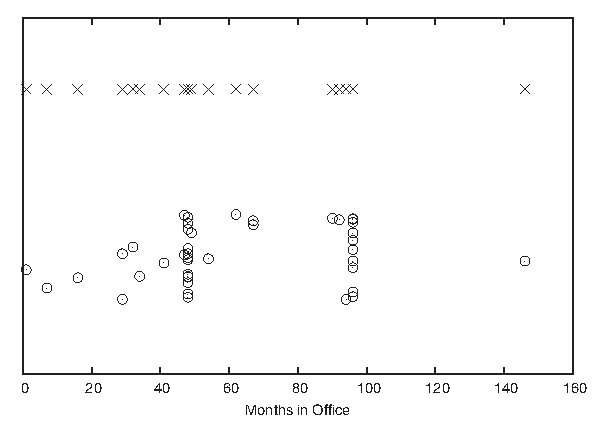
\includegraphics{img/presidents}}
  \caption{Dot and jitter plots showing the number of months U.S.\
    presidents spent in office.}
  \label{fig:presidents}
\end{figure}

What does the jitter plot tell us about the data set?  We see two
values where data points seem to cluster, indicating that these values
occur more frequently than others. Not surprisingly, they are located
at 48 and 96 months, which correspond to one and two full four-year
terms in office. What may be a little surprising, however, is the
relatively large number of points that occur \emph{outside} these
clusters.  Apparently, quite a few presidents left office at irregular
intervals!  Even in this simple example, a plot reveals both something
expected (the clusters at 48 and 96 months) and the unexpected (the
larger number of points outside those clusters).

Before moving on to our second example, let me point out a few
additional technical details regarding jitter plots.

\begin{itemize}
\item It is important that the amount of ``jitter'' be small compared
  to the distance between points. The only purpose of the random
  displacements is to ensure that no two points fall exactly on top of
  one another. We must make sure that points are not shifted
  significantly from their true location.

\item We can jitter points in either the horizontal or the vertical
  direction (or both), depending on the data set and the purpose of
  the graph. In Figure \ref{fig:presidents}, points were jittered only
  in the vertical direction, so that their horizontal position (which
  in this case corresponds to the actual data---namely, the number of
  months in office) is not altered and therefore remains exact.

\item I used open, transparent rings as symbols for the data points.
  This is no accident: among different symbols of equal size, open
  rings are most easily recognized as separate even when partially
  occluded by each other. In contrast, filled symbols tend to hide
  any substructure when they overlap, and symbols made from straight
  lines (\eg,\ boxes and crosses) can be confusing because of the large
  number of parallel lines; see the top part of Figure
  \ref{fig:presidents}.
\end{itemize}

Jittering is a good trick that can be used in many different contexts.
We will see further examples later in the book.


% ============================================================
\section{Histograms and Kernel Density Estimates}

\index{univariate analysis!histograms and kernel density estimates|(} 

Dot and jitter plots are nice because they are so simple.  However,
they are neither pretty nor very intuitive, and most importantly, they
make it hard to read off \emph{quantitative} information from the
graph. In particular, if we are dealing with larger data sets, then we
need a better type of graph, such as a histogram.

\subsection{Histograms}

\index{histograms!about|(}
 
To form a \emph{histogram}, we divide the range of values into a set
of ``bins'' and then count the number of points (sometimes called
``events'') that fall into each bin. We then plot the count of events
for each bin as a function of the position of the bin.

Once again, let's look at an example. Here is the beginning of a file
containing response times (in milliseconds) for queries against a web
server or database. In contrast to the previous example, this data
set is fairly large, containing 1,000 data points.

\begin{verbatim}
 452.42
 318.58
 144.82
 129.13
1216.45
 991.56
1476.69
 662.73
1302.85
1278.55
 627.65
1030.78
 215.23
  44.50
...
\end{verbatim}

Figure \ref{fig:serverhisto} shows a histogram of this data set. I
divided the horizontal axis into 60 bins of 50 milliseconds width and
then counted the number of events in each bin.

\begin{figure}
  \centerline{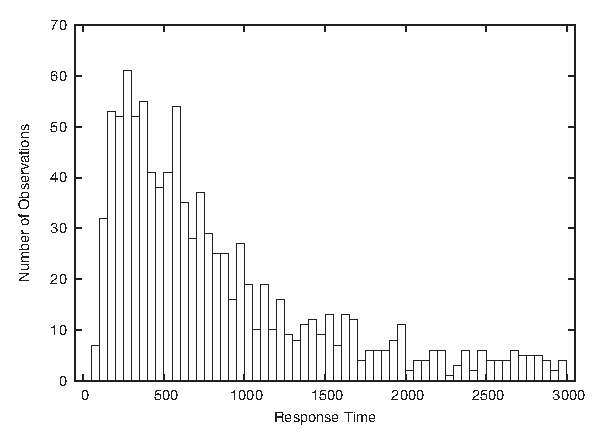
\includegraphics{img/server-data-histo}}
  \caption{A histogram of a server's response times.}
  \label{fig:serverhisto}
\end{figure}\pagebreak

What does the histogram tell us? We observe a rather sharp cutoff at a
nonzero value on the left, which means that there is a minimum
completion time below which no request can be completed. Then there is
a sharp rise to a maximum at the ``typical'' response time, and
finally there is a relatively large tail on the right, corresponding
to the smaller number of requests that take a long time to process.
This kind of shape is rather typical for a histogram of task
completion times.  If the data set had contained completion times for
students to finish their homework or for manufacturing workers to
finish a work product, then it would look qualitatively similar
except, of course, that the time scale would be different. Basically,
there is some minimum time that nobody can beat, a small group of very
fast champions, a large majority, and finally a longer or shorter tail
of ``stragglers.''

It is important to realize that a data set does not determine a
histogram uniquely. Instead, we have to fix \emph{two} parameters to
form a histogram: the bin width and the alignment of the bins.

The quality of any histogram hinges on the proper choice of bin width.
If you make the width too large, then you lose too much detailed
information about the data set. Make it too small and you will have
few or no events in most of the bins, and the shape of the distribution
does not become apparent. Unfortunately, there is no simple rule of
thumb that can predict a good bin width for a given data set;
typically you have to try out several different values for the bin
width until you obtain a satisfactory result. (As a first guess, you
can start with \emph{Scott's rule} for the bin width $w = 3.5 \sigma /
\sqrt[3]{n}$, where $\sigma$ is the standard deviation for the entire
data set and $n$ is the number of points. This rule assumes that the
data follows a Gaussian distribution;\index{Gaussian distribution (Gaussian function)!histograms} otherwise, it is likely to give
a bin width that is too wide. See the end of this chapter for more
information on the standard deviation.)

The other parameter that we need to fix (whether we realize it or
not) is the alignment of the bins on the $x$ axis. Let's say we fixed
the width of the bins at $1$.  Where do we now place the first bin? We
could put it flush left, so that its left edge is at $0$, or we could
center it at $0$. In fact, we can move all bins by half a bin width
in either direction.

Unfortunately, this seemingly insignificant (and often overlooked)
parameter can have a large influence on the appearance of the
histogram.  Consider this small data set:

\begin{verbatim}
1.4
1.7
1.8
1.9
2.1
2.2
2.3
2.6
\end{verbatim}

Figure \ref{fig:smallhisto} shows two histograms of this data set.
Both use the same bin width (namely, $1$) but have different
alignment of the bins. In the top panel, where the bin \emph{edges}
have been aligned to coincide with the whole numbers ($1, 2, 3,
\dots$), the data set appears to be flat. Yet in the bottom panel,
where the bins have been\vadjust{\pagebreak} \emph{centered} on the whole numbers, the
data set appears to have a rather strong central peak and symmetric
wings on both sides.  It should be clear that we can construct even
more pathological examples than this. In the next section we shall
introduce an alternative to histograms that avoids this particular
problem.

\begin{figure}
  \centerline{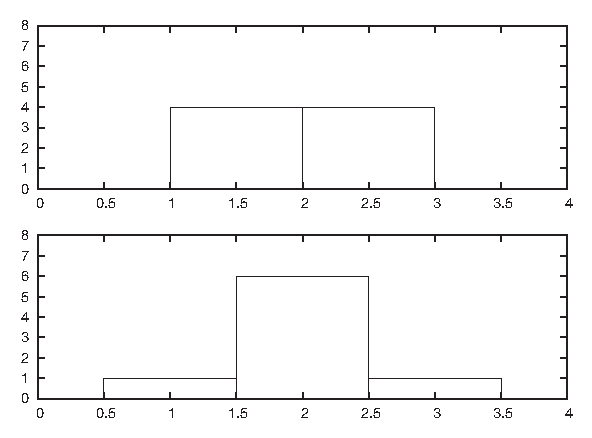
\includegraphics{img/small-histo}}
  \caption{Histograms can look quite different, depending on the
    choice of anchoring point for the first bin. The figure shows
    two histograms of the same data set, using the same bin width.
    In the top panel, the bin edges are aligned on whole numbers;
    in the bottom panel, bins are centered on whole numbers.}
  \label{fig:smallhisto}
\end{figure}

Before moving on, I'd like to point out some additional technical
details and variants of histograms.

\begin{itemize}
\item Histograms can be either normalized or unnormalized.\index{normalized histograms} \index{unnormalized histograms} In an
  \emph{unnormalized} histogram, the value plotted for each bin is the
  absolute count of events in that bin. In a \emph{normalized}
  histogram, we divide each count by the total number of points in the
  data set, so that the value for each bin becomes the fraction of
  points in that bin. If we want the percentage of points per bin
  instead, we simply multiply the fraction by $100$.

\item So far I have assumed that all bins have the same width.  We can
  relax this constraint and allow bins of differing widths---narrower
  where points are tightly clustered but wider in areas where there
  are only few points. This method can seem very appealing when the
  data set has outliers or areas with widely differing point density.
  Be warned, though, that now there is an additional source of
  ambiguity for your histogram: should you display the absolute number
  of points per bin regardless of the width of each bin; or should you
  display the density of points per bin by normalizing the point count
  per bin by the bin width?  Either method is valid, and you cannot
  assume that your audience will know which convention you are
  following.\pagebreak

\item It is customary to show histograms with rectangular boxes that
  extend from the horizontal axis, the way I have drawn Figures
  \ref{fig:serverhisto} and \ref{fig:smallhisto}.  That is perfectly
  all right and has the advantage of explicitly displaying the bin
  width as well. (Of course, the boxes should be drawn in such a way
  that they align in the same way that the actual bins align; see
  Figure \ref{fig:smallhisto}.) This works well if you are only
  displaying a histogram for a single data set. But if you want to
  compare two or more data sets, then the boxes start to get in the
  way, and you are better off drawing ``frequency polygons'': eliminate
  the boxes, and instead draw a symbol where the top of the box would
  have been.  (The horizontal position of the symbol should be at the
  center of the bin.) Then connect consecutive symbols with straight
  lines.  Now you can draw multiple data sets in the same plot
  without cluttering the graph or unnecessarily occluding points.
  % --- XXX : Reference to a freq polygon elsewhere in the text?

\item Don't assume that the defaults of your graphics program will
  generate the best representation of a histogram! I have already
  discussed why I consider frequency polygons to be almost always a
  better choice than to construct a histogram from boxes.  If you
  nevertheless choose to use boxes, it is best to avoid filling them
  (with a color or hatch pattern)---your histogram will probably look
  cleaner and be easier to read if you stick with just the box
  outlines. Finally, if you want to compare several data sets in the
  same graph, always use a frequency polygon, and stay away from
  stacked or clustered bar graphs, since these are particularly hard
  to read. (We will return to the problem of displaying composition
  problems in Chapter \ref{ch:multivariate}.)
\end{itemize}

Histograms are very common and have a nice, intuitive interpretation.
They are also easy to generate: for a moderately sized data set, it
can even be done by hand, if necessary.  That being said, histograms
have some serious problems.  The most important ones are as follows.

\begin{itemize}
\item The binning process required by all histograms loses information
  (by replacing the location of individual data points with a bin of
  finite width). If we only have a few data points, we can ill afford
  to lose any information.

\item Histograms are not unique. As we saw in Figure
  \ref{fig:smallhisto}, the appearance of a histogram can be quite
  different. (This nonuniqueness is a direct consequence of the
  information loss described in the previous item.)

\item On a more superficial level, histograms are ragged and not
  smooth.  This matters little if we just want to draw a picture of
  them, but if we want to feed them back into a computer as input for
  further calculations, then a smooth curve would be easier to handle.

\item Histograms do not handle outliers gracefully. A single outlier,
  far removed from the majority of the points, requires many empty
  cells in between or forces us to use bins that are too wide for the
  majority of points. It is the possibility of outliers that makes it
  difficult to find an acceptable bin width in an automated fashion.
\end{itemize}

Fortunately, there is an alternative to classical histograms that has
none of these problems. It is called a \emph{kernel density estimate}.

\index{histograms!about|)}

% ============================================================
\subsection{Kernel Density Estimates}

\index{kernel density estimates|(} 

Kernel density estimates (KDEs) are a relatively new technique. In
contrast to histograms, and to many other classical methods of data
analysis, they pretty much \emph{require} the calculational power of a
reasonably modern computer to be effective. They cannot be done ``by
hand'' with paper and pencil, even for rather moderately sized data
sets. (It is interesting to see how the accessibility of computational
and graphing power enables new ways to think about data!)

To form a KDE, we place a \emph{kernel}---that is, a smooth, strongly
peaked function---at the position of each data point. We then add up
the contributions from all kernels to obtain a smooth curve, which we
can evaluate at any point along the $x$ axis.

Figure \ref{fig:presidentskde} shows an example. This is yet another
representation of the data set we have seen before in Figure
\ref{fig:presidents}. The dotted boxes are a histogram of the data
set (with bin width equal to $1$), and the solid curves are two KDEs
of the same data set with different bandwidths (I'll explain this
concept in a moment). \index{bandwidth selection, KDEs} The shape of the individual kernel functions can
be seen clearly---for example, by considering the three data points
below $20$. You can also see how the final curve is composed out of
the individual kernels, in particular when you look at the points
between $30$ and $40$.

\begin{figure}
  \centerline{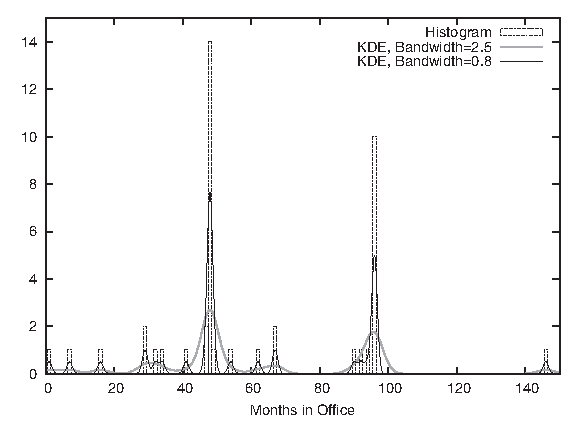
\includegraphics{img/presidents-kde}}
  \caption{Histogram and kernel density estimate of the distribution
    of the time U.S.\ presidents have spent in office.}
  \label{fig:presidentskde}
\end{figure}\pagebreak

We can use any smooth, strongly peaked function as a kernel provided
that it integrates to $1$; in other words, the area under the curve
formed by a single kernel must be $1$. (This is necessary to make sure
that the resulting KDE is properly normalized.) Some examples of
frequently used kernel functions include (see Figure
\ref{fig:kernels}):
%
\begin{align*}
K(x) & = 
\begin{cases}
  \frac{1}{2} & \text{if $\abs{x} \le 1$} \\
  0           & \text{otherwise}
\end{cases}
     & \text{box or boxcar kernel} \\
K(x) & = 
\begin{cases}
  \frac{3}{4} \paren{1-x^2} & \text{if $\abs{x} \le 1$} \\
  0                         & \text{otherwise}
\end{cases}
     & \text{Epanechnikov kernel} \\
K(x) & = \frac{1}{\sqrt{2 \pi}} \exp\paren{- \frac{1}{2} x^2}
     & \text{Gaussian kernel}
\end{align*}
%
The box kernel and the Epanechnikov kernel are zero outside a finite
range, whereas the Gaussian kernel \index{Gaussian distribution (Gaussian function)!KDEs} is nonzero everywhere but
negligibly small outside a limited domain. It turns out that the curve
resulting from the KDE does not depend strongly on the particular
choice of kernel function, so we are free to use the kernel that is
most convenient.  Because it is so easy to work with, the Gaussian
kernel is the most widely used. (See Appendix \ref{app:calculus} for
more information on the Gaussian function.)

\begin{figure}
  \centerline{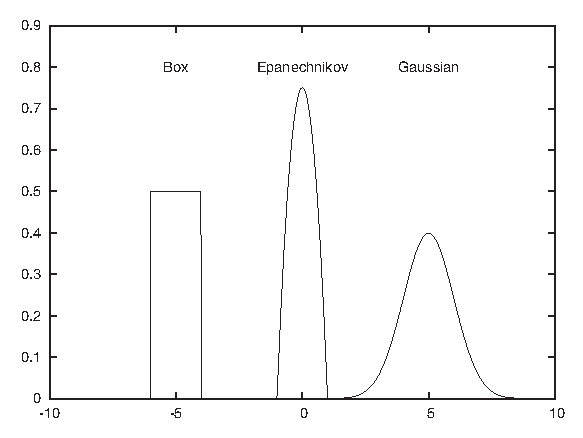
\includegraphics{img/kernels}}
  \caption{Graphs of some frequently used kernel functions.}
  \label{fig:kernels}
\end{figure}


Constructing a KDE requires to things: first, we must move the kernel
to the position of each point by shifting it appropriately.  For
example, the function $K( x - x_i )$ will have its peak at $x_i$, not
at $0$.  Second, we have to choose the kernel \emph{bandwidth},
which controls the spread of the kernel function. To make sure that
the area under the curve stays the same as we shrink the width, we
have to make the curve higher\vadjust{\pagebreak} (and lower if we increase the width).
The final expression for the shifted, rescaled kernel function of
bandwidth $h$ is:
%
\[
\frac{1}{h} K\paren{ \frac{x-x_i}{h} }
\]
%
This function has a peak at $x_i$, its width is approximately $h$, and
its height is such that the area under the curve is still $1$.  Figure
\ref{fig:gausskernel} shows some examples, using the Gaussian kernel.
Keep in mind that the area under all three curves is the same.

\begin{figure}
  \centerline{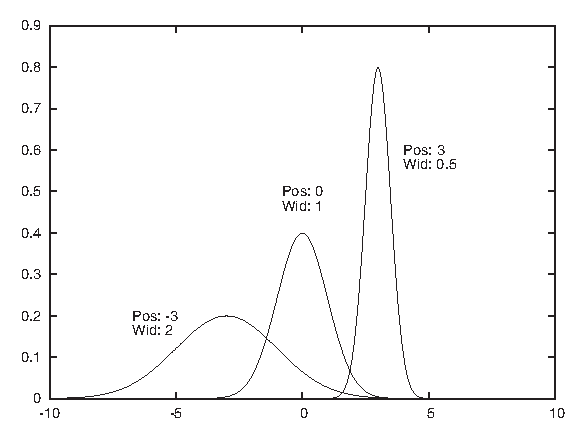
\includegraphics{img/gauss-kernel}}
  \caption{The Gaussian kernel for three different bandwidths.  The
    height of the kernel increases as the width decreases, so the
    total area under the curve remains constant.}
  \label{fig:gausskernel}
\end{figure}

Using this expression, we can now write down a formula for the KDE
with bandwidth $h$ for any data set $\braces{ x_1, x_2, \dots, x_n }$.
This formula can be evaluated for any point $x$ along the $x$ axis:
%
\[
D_h\paren{ x; \braces{ x_i } } 
  = \sum_{i=1}^n \frac{1}{h} K\paren{ \frac{x-x_i}{h} }
\]
%
All of this is straightforward and easy to implement in any computer
language. Be aware that for large data sets (those with many thousands
of points), the required number of kernel evaluations can lead to
performance issues, especially if the function $D(x)$ needs to be
evaluated for many different positions (\ie, many different values of
$x$). If this becomes a problem for you, you may want to choose a
simpler kernel function or not evaluate a kernel if the distance
$x-x_i$ is significantly greater than the bandwidth $h$.\footnote{Yet another strategy starts with the realization that
  forming a KDE amounts to a convolution of the kernel function with
  the data set. You can now take the Fourier transform of both kernel
  and data set and make use of the Fourier convolution theorem.  This
  approach is suitable for very large data sets but is outside the
  scope of our discussion.}

Now we can explain the wide gray line in Figure
\ref{fig:presidentskde}: it is a KDE with a larger bandwidth. Using
such a large bandwidth makes it impossible to resolve the individual
data points, but it does highlight entire \emph{periods} of greater or
smaller frequency. Which choice of bandwidth is right for you depends
on your purpose.

A KDE constructed as just described is similar to a classical
histogram, but it avoids two of the aforementioned problems.  Given
data set and bandwidth, a KDE is unique; a KDE is also smooth,
provided we have chosen a smooth kernel function, such as the
Gaussian.

\vspace*{-6pt}
\subsection{Optional: Optimal Bandwidth Selection}

\index{bandwidth selection, KDEs}
\index{histograms!bandwidth selection}

We still have to fix the bandwidth. This is a different \emph{kind} of
problem than the other two: it's not just a technical problem, which
could be resolved through a better method; instead, it's a fundamental
problem that relates to the data set itself.  If the data follows a
smooth distribution, then a wider bandwidth is appropriate, but if the
data follows a very wiggly distribution, then we need a smaller
bandwidth to retain all relevant detail. In other words, the optimal
bandwidth is a property of the data set and tells us something about
the nature of the data.

So how do we choose an optimal value for the bandwidth?  Intuitively,
the problem is clear: we want the bandwidth to be narrow enough to
retain all relevant detail but wide enough so that the resulting curve
is not too ``wiggly.'' This is a problem that arises in every
approximation problem: balancing the faithfulness of representation
against the simplicity of behavior. Statisticians speak of the
``bias--variance trade-off.''

To make matters concrete, we have to define a specific expression for
the error of our approximation, one that takes into account both bias
and variance. We can then choose a value for the bandwidth that
minimizes this error. For KDEs, the generally accepted measure is the
``expected mean-square error''\index{mean-square error, KDE bandwidth}  between the approximation and the true
density.  The problem is that we don't know the true density function
that we are trying to approximate, so it seems impossible to calculate
(and minimize) the error in this way. But clever methods have been
developed to make progress. These methods fall broadly into two
categories. First, we could try to find explicit expressions for
both bias and variance.  Balancing them leads to an equation that has
to be solved numerically or---if we make additional assumptions (\eg,
that the distribution is Gaussian)---can even yield explicit
expressions similar to Scott's rule (introduced earlier when talking
about histograms).  Alternatively, we could realize that the KDE is an
approximation for the probability density from which the original set
of points was chosen. We can therefore choose points from this
approximation (\ie, from the probability density represented by
the KDE) and see how well they replicate the KDE that we started with.
Now we change the bandwidth until we find that value for which the KDE
is best replicated: the result is the estimate of the ``true''
bandwidth of the data. (This latter method is known as
\emph{cross-validation}.)

Although not particularly hard, the details of both methods would lead
us too far afield, and so I will skip them here.\vadjust{\pagebreak}  If you are
interested, you will have no problem picking up the details from one
of the references at the end of this chapter.  Keep in mind, however,
that these methods find the optimal bandwidth \emph{with respect to
  the mean-square error}, which tends to overemphasize bias over variance and therefore
these methods lead to rather narrow bandwidths and KDEs that appear
too wiggly. If you are using KDEs to generate graphs for
the purpose of obtaining intuitive visualizations of point
distributions, then you might be better off with a bit of manual trial
and error combined with visual inspection.  In the end, there is no
``right'' answer, only the most suitable one for a given purpose.
Also, the most suitable to develop intuitive understanding might not
be the one that minimizes a particular mathematical quantity.

\index{univariate analysis!histograms and kernel density estimates|)} 
\index{kernel density estimates|)} 

% ============================================================
\section{The Cumulative Distribution Function}

\index{univariate analysis!cumulative distribution function|(}
\index{CDF (cumulative distribution function)|(} 
\index{cumulative distribution function (CDF)|(} 
  
The main advantage of histograms and kernel density estimates is that
they have an immediate intuitive appeal: they tell us how probable it
is to find a data point with a certain value. For example, from Figure
\ref{fig:serverhisto} it is immediately clear that values around 250
milliseconds are very likely to occur, whereas values greater than
2,000 milliseconds are quite rare.

But how rare, exactly? That is a question that is much harder to
answer by looking at the histogram in Figure \ref{fig:serverhisto}.
Besides wanting to know how much weight is in the tail, we might also
be interested to know what fraction of requests completes in the
typical band between 150 and 350 milliseconds. It's certainly the
majority of events, but if we want to know exactly how many, then we
need to sum up the contributions from all bins in that region.

The \emph{cumulative distribution function} (CDF) does just that. The CDF at
point $x$ tells us what fraction of events has occurred ``to the
left'' of $x$. In other words, the CDF is the fraction of all points
$x_i$ with $x_i \le x$.

Figure \ref{fig:serverkde} shows the same data set that we have
already encountered in Figure \ref{fig:serverhisto}, but here the data
is represented by a KDE (with bandwidth $h=30$) instead of a
histogram. In addition, the figure also includes the corresponding
CDF.  (Both KDE and CDF are normalized to $1$.)

\begin{figure}
  \centerline{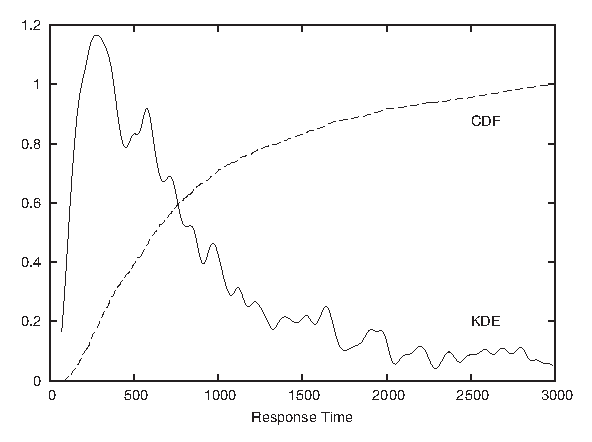
\includegraphics{img/server-data-kde}}
  \caption{Kernel density estimate and cumulative distribution
    function of the server response times shown\break in Figure
    \ref{fig:serverhisto}.}\label{fig:serverkde}
\end{figure}

We can read off several interesting observations directly from the
plot of the CDF. For instance, we can see that at $t=\text{1,500}$
(which certainly puts us into the tail of the distribution) the CDF is
still smaller than $0.85$; this means that fully 15 percent of all
requests take longer than 1,500 milliseconds. In contrast, less than a
third of all requests are completed in the ``typical'' range of
150--500 milliseconds.  (How do we know this? The CDF for $t=150$ is
about $0.05$ and is close to $0.40$ for $t=500$. In other words, about
40 percent of all requests are completed in less than $500$
milliseconds; of these, 5 percent are completed in less than $150$
milliseconds.  Hence about 35 percent of all requests have response
times of between $150$ and $500$ milliseconds.)

It is worth pausing to contemplate these findings, because they
demonstrate how misleading a histogram (or KDE) can be despite (or
because of) their intuitive appeal! Judging from the histogram or KDE
alone, it seems quite reasonable to assume that ``most'' of the events
occur within the major peak near $t=300$ and that the tail for $t >
\text{1,500}$ contributes relatively little. Yet the CDF tells us
clearly that this is not so. (The problem is that the eye is much
better at judging distances than areas, and we are therefore misled by
the large values of the histogram near its peak and fail to see that
nevertheless the area beneath the peak is not that large compared to
the total area under the curve.)

CDFs are probably the least well-known and most underappreciated tool
in basic graphical analysis. They have less immediate intuitive appeal
than histograms or KDEs, but they allow us to make the kind of
quantitative statement that is very often required but is
difficult (if not impossible) to obtain from a histogram.

Cumulative distribution functions have a number of important
properties that follow directly from how they are calculated.

\begin{itemize}
\item Because the value of the CDF at position $x$ is the fraction of
  points to the left of $x$, a CDF is always monotonically increasing
  with $x$.

\item CDFs are less wiggly than a histogram (or KDE) but contain the
  same information in a representation that is inherently less noisy.

\item Because CDFs do not involve any binning, they do not lose
  information and are therefore a more faithful representation of the
  data than a histogram.

\item All CDFs approach $0$ as $x$ goes to negative infinity. CDFs
  are usually normalized so that they approach $1$ (or 100 percent) as
  $x$ goes to positive infinity.

\item A CDF is unique for a given data set.
\end{itemize}

If you are mathematically inclined, you have probably already realized
that the CDF is (an approximation to) the antiderivative of the
histogram and that the histogram is the derivative of the CDF:\vspace*{-3pt}
%
\begin{gather*}
\operatorname{cdf}(x) 
  \approx \int_{-\infty}^{x} \lms{t} \operatorname{histo}(t) \\
\operatorname{histo}(x) 
  \approx \Diff{x} \operatorname{cdf}(x)
\end{gather*}
%
Cumulative distribution functions have several uses. First, and most
importantly, they enable us to answer questions such as those posed
earlier in this section: what fraction of points falls between any two
values? The answer can simply be read off from the graph. Second, CDFs
also help us understand how imbalanced a distribution is---in other
words, what fraction of the overall weight is carried by the tails.

Cumulative distribution functions also prove useful when we want to
compare two distributions. It is notoriously difficult to compare two
bell-shaped curves in a histogram against each other. Comparing the
corresponding CDFs is usually much more conclusive.

One last remark, before leaving this section: in the literature, you
may find the term \emph{quantile plot}.\index{quantile plots}  A quantile plot is just the
plot of a CDF in which the $x$ and $y$ axes have been switched.
Figure \ref{fig:serverquantile} shows an example using once again the
server response time data set. Plotted this way, we can easily answer
questions such as, ``What response time corresponds to the 10th
percentile of response times?''  But the information contained in this
graph is of course exactly the same as in a graph of the CDF.

\begin{figure}
  \centerline{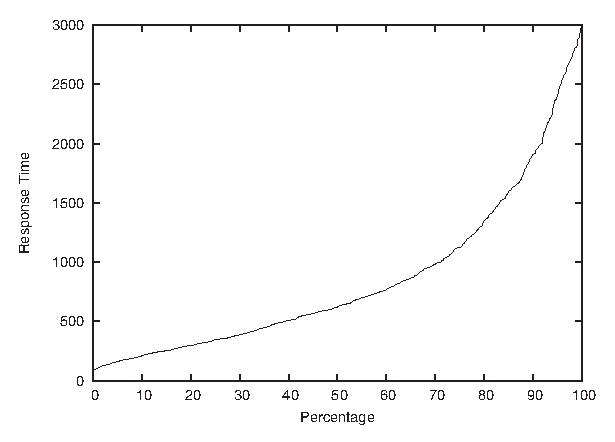
\includegraphics{img/serverquantile}}
  \caption{Quantile plot of the server data. A quantile plot is a
    graph of the CDF with the $x$ and $y$ axes interchanged. Compare
    to Figure \ref{fig:serverkde}.}
  \label{fig:serverquantile}
\end{figure}

\vspace*{-6pt}
\subsection{Optional: Comparing Distributions with Probability Plots and QQ Plots}

\index{probability plots, comparing with distributions|(}
\index{QQ plots!comparing with distributions|(}

Occasionally you might want to confirm that a given set of points 
is distributed according to some specific, known distribution. For
example, you have a data set and would like to determine whether it
can be described well by a Gaussian (or some other) distribution.

% --- XXX : not yet explained: density function. Does it matter?
You could compare a histogram or KDE of the data set directly against
the theoretical density function, but it is notoriously difficult to
compare distributions that way---especially out in the tails.  A
better idea would be to compare the cumulative distribution functions,
which are easier to handle because they are less wiggly and are always
monotonically increasing. But this is still not easy. Also keep in
mind that most probability distributions depend on location and scale
parameters (such as mean and variance), which you would have to
estimate \emph{before} being able to make a meaningful comparison.
Isn't there a way to compare a set of points directly against a
theoretical distribution and, in the process, read off the estimates
for all the parameters required?

As it turns out, there is. The method is technically easy to do, but
the underlying logic is a bit convoluted and tends to trip up even
experienced practitioners.


\begin{figure}
  \centerline{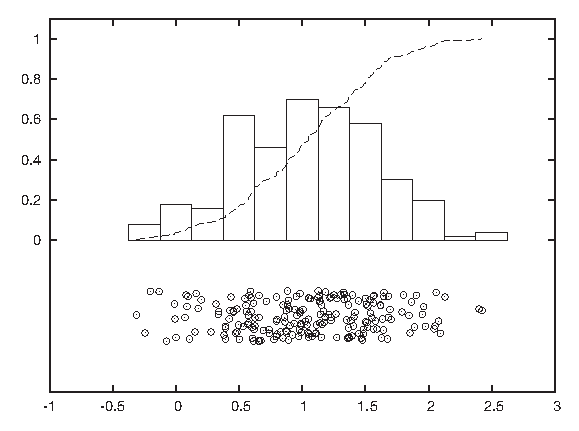
\includegraphics{img/happyqq1}}
  \caption{Jitter plot, histogram, and cumulative distribution function
    for a Gaussian data set.}
  \label{fig:happyqq1}
\end{figure}

Here is how it works. Consider a set of points $\braces{x_i}$ that we
suspect are distributed according to the Gaussian distribution. In 
other words, we expect the cumulative distribution function of the
set\vadjust{\pagebreak} of points, $y_i = \operatorname{cdf}(x_i)$, to be the Gaussian 
cumulative distribution function $\Phi\paren{ (x-\mu)/\sigma }$
with mean $\mu$ and standard deviation $\sigma$:
%
\[
y_i = \Phi\paren{ \frac{x_i-\mu}{\sigma } } 
  \quad \text{only if data is Gaussian}
\]
%
Here, $y_i$ is the value of the cumulative distribution function 
corresponding to the data point $x_i$; in other words, $y_i$ is
the \emph{quantile} of the point $x_i$.

Now comes the trick. We apply the \emph{inverse} of the Gaussian
distribution function to both sides of the equation:
%
\[
\Phi^{-1}(y_i) = \frac{x_i-\mu}{\sigma }
\]
%
With a little bit of algebra, this becomes
%
\[
x_i = \mu + \sigma \Phi^{-1}(y_i)
\]
%
In other words, if we plot the values in the data set as a function of
$\Phi^{-1}(y_i)$, then they should fall onto a straight line with
slope $\sigma$ and zero intercept $\mu$. If, on the other hand, the
points do not fall onto a straight line after applying the inverse
transform, then we can conclude that the data is not distributed
according to a Gaussian distribution.

\begin{figure}
  \centerline{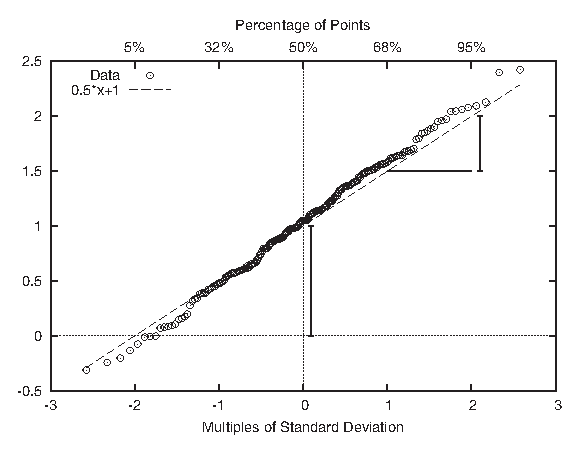
\includegraphics{img/happyqq2}}
  \caption{Probability plot for the data set shown in Figure 
    \ref{fig:happyqq1}.}
  \label{fig:happyqq2}
\end{figure}

The resulting plot is known as a \emph{probability plot}. Because it
is easy to spot deviation from a straight line, a probability plot
provides a relatively sensitive test to determine whether a set of
points behaves according to the Gaussian distribution. As an added
benefit, we can read off estimates for the mean and the standard
deviation directly from the graph: $\mu$ is the intercept of the curve
with the $y$ axis, and $\sigma$ is given by the slope of the curve.
(Figure \ref{fig:happyqq2} shows the probability plot for the Gaussian
data set displayed in Figure \ref{fig:happyqq1}.)

One important question concerns the \emph{units} that we plot along
the axes. For the vertical axis the case is clear: we use whatever
units the original data was measured in. But what about the horizontal
axis? We plot the data as a function of $\Phi^{-1}(y_i)$, which is the
inverse Gaussian distribution function, applied to the percentile
$y_i$ for each point $x_i$. We can therefore choose between two
different ways to dissect the horizontal axis: either using the
percentiles $y_i$ directly (in which case the tick marks will not be
distributed uniformly), or dividing the horizontal axis uniformly. In
the latter case we are using \emph{the width of the standard Gaussian
  distribution} as a unit. You can convince yourself that this is
really true by realizing that $\Phi^{-1}(y)$ is the inverse of the
Gaussian distribution function $\Phi(x)$. Now ask yourself: what units
is $x$ measured in? We use the same units for the horizontal axis of a
Gaussian probability plot.  These units are sometimes called
\emph{probits}. (Figure \ref{fig:happyqq2} shows both sets of units.)
Beware of confused and confusing explanations of this point elsewhere
in the literature.

There is one more technical detail that we need to discuss: to produce
a probability plot, we need not only the data itself, but for each
point $x_i$ we also need its quantile $y_i$ (we will discuss
quantiles and percentiles in more detail later in this chapter). The
simplest way to obtain the quantiles, given the data, is as follows:

\begin{enumerate}
\item Sort the data points in ascending order.
\item Assign to each data point its rank (basically, its line number
  in the sorted file), starting at $1$ (not at $0$).
\item The quantile $y_i$ now is the rank divided by $n+1$, where
  $n$ is the number of data points.
\end{enumerate}

This prescription guarantees that each data point is assigned a
quantile that is strictly greater than $0$ and strictly less than $1$.
This is important because $\Phi^{-1}(x)$ is defined only for $0 < x <
1$. This prescription is easy to understand and easy to remember, but
you may find other, slightly more complicated prescriptions elsewhere.
For all practical purposes, the differences are going to be small.

Finally, let's look at an example where the data is clearly \emph{not}
Gaussian. Figure \ref{fig:serverdataqq} shows the server data from
Figure \ref{fig:serverhisto} plotted in a probability plot.  The
points don't fall on a straight line at all---which is no surprise
since we already knew from Figure \ref{fig:serverhisto} that the data
is not Gaussian.  But for cases that are less clear-cut, the
probability plot can be a helpful tool for detecting deviations from
Gaussian behavior.
% Long tails: data in tails ``steeper'' than straight line
% Short tails: data in tails ``flatter'' than straight line

\begin{figure}
  \centerline{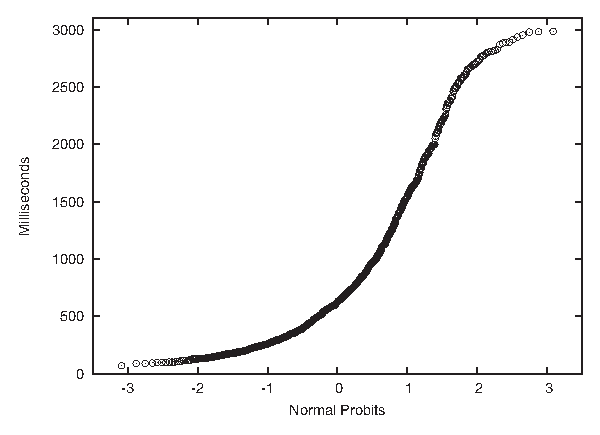
\includegraphics{img/serverdataqq}}
  \caption{A probability plot of the server response times from Figure
    \ref{fig:serverhisto}. The data does not follow a Gaussian
    distribution and thus the points do \emph{not} fall on a straight
    line.}
  \label{fig:serverdataqq}
\end{figure}

A few additional comments are in order here.

\begin{itemize}
\item Nothing in the previous discussion requires that the
  distribution be Gaussian! You can use almost any other commonly used
  distribution function (and its inverse) to generate the respective
  probability plots. In particular, many of the commonly used\vadjust{\vfill\pagebreak}
  probability distributions depend on location and scale parameters in
  exactly the same way as the Gaussian distribution, so all the
  arguments discussed earlier go through as before.
\item So far, I have always assumed that we want to compare an
  \emph{empirical} data set against a \emph{theoretical} distribution.
  But there may also be situations where we want to compare two
  empirical data sets against each other---for example, to find out
  whether they were drawn from the same family of distributions
  (without having to specify the family explicitly). The process is
  easiest to understand when both data sets we want to compare contain
  the same number of points. You sort both sets and then align the
  points from both data sets that have the same rank (once sorted).
  Now plot the resulting pairs of points in a regular scatter plot
  (see Chapter \ref{ch:bivariate}); the resulting graph is known as a
  \emph{QQ plot}. (If the two data sets do not contain the same number
  of points, you will have to interpolate or truncate them so that
  they do.)
\end{itemize}

Probability plots are a relatively advanced, specialized technique,
and you should evaluate whether you really need them. Their purpose is
to determine whether a given data set stems from a specific, known
distribution. Occasionally, this is of interest in itself; in other
situations subsequent analysis depends on proper identification of the
underlying model. For example, many statistical techniques assume that
the errors or residuals are Gaussian and are not applicable if this
condition is violated.  Probability plots are a convenient technique
for testing this assumption.
\index{univariate analysis!cumulative distribution function|)}
\index{CDF (cumulative distribution function)|)} 
\index{cumulative distribution function (CDF)|)} 
\index{probability plots, comparing with distributions|)}
\index{QQ plots!comparing with distributions|)}\vfill\pagebreak

% ============================================================
\section{Rank-Order Plots and Lift Charts}

\index{univariate analysis!rank-order plots and lift charts|(}
\index{rank-order plots|(}
\index{lift charts|(}

There is a technique related to histograms and CDFs that is worth
knowing about. Consider the following scenario. A company that is
selling textbooks and other curriculum materials is planning an email
marketing campaign to reach out to its existing customers.  For this
campaign, the company wants to use personalized email messages that
are tailored to the job title of each recipient (so that teachers will
receive a different email than their principals).  The problem is the
customer database contains about 250,000 individual customer records
with over 16,000 different job titles among them! Now what?

The trick is to sort the job titles by the number of individual
customer records corresponding to each job title. The first few
records are shown in Table \ref{tbl:jobtitles}. The four columns give
the job title, the number of customers for that job title, the
fraction of all customers having that job title, and finally the
cumulative fraction of customers. For the last column, we sum up the
number of customers for the current and all previously seen job
titles, then divide by the total number of customer records. This is
the equivalent of the CDF we discussed earlier.

We can see immediately that fully two thirds of all customers account
for only 10 different job titles. Using just the top 30 job titles
gives us 75 percent coverage of customer records. That's much more
manageable than the 16,000 job titles we started with!

\begin{table}
\newlength{\unicola}
\newlength{\unicolb}
\newlength{\unicolc}
\settowidth{\unicola}{Number ofX}
\settowidth{\unicolb}{Fraction ofX}
\settowidth{\unicolc}{Cumulative}
\tbl{The first 30 job titles and their relative frequencies.\label{tbl:jobtitles}}{%
\begin{tabular}{lrrr}
\toprule
   & \textbf{Number of}
   & \textbf{Fraction of}
  & \textbf{Cumulative} \\
\textbf{Title} &  \textbf{customers} & \textbf{customers} & \textbf{fraction}\\
\colrule
Teacher \rule{0mm}{4mm}  & 66,470  &  0.34047   &   0.340 \\ 
Principal                & 22,958  &  0.11759   &   0.458 \\
Superintendent           & 12,521  &  0.06413   &   0.522 \\
Director                 & 12,202  &  0.06250   &   0.584 \\
Secretary                &  4,427  &  0.02267   &   0.607 \\
Coordinator              &  3,201  &  0.01639   &   0.623 \\
Vice Principal           &  2,771  &  0.01419   &   0.637 \\
Program Director         &  1,926  &  0.00986   &   0.647 \\
Program Coordinator      &  1,718  &  0.00880   &   0.656 \\
Student                  &  1,596  &  0.00817   &   0.664 \\
Consultant               &  1,440  &  0.00737   &   0.672 \\
Administrator            &  1,169  &  0.00598   &   0.678 \\
President                &  1,114  &  0.00570   &   0.683 \\
Program Manager          &  1,063  &  0.00544   &   0.689 \\
Supervisor               &  1,009  &  0.00516   &   0.694 \\
Professor                &    961  &  0.00492   &   0.699 \\
Librarian                &    940  &  0.00481   &   0.704 \\
Project Coordinator      &    880  &  0.00450   &   0.708 \\
Project Director         &    866  &  0.00443   &   0.713 \\
Office Manager           &    839  &  0.00429   &   0.717 \\
Assistant Director       &    773  &  0.00395   &   0.721 \\
Administrative Assistant &    724  &  0.00370   &   0.725 \\
Bookkeeper               &    697  &  0.00357   &   0.728 \\
Intern                   &    693  &  0.00354   &   0.732 \\
Program Supervisor       &    602  &  0.00308   &   0.735 \\
Lead Teacher             &    587  &  0.00300   &   0.738 \\
Instructor               &    580  &  0.00297   &   0.741 \\
Head Teacher             &    572  &  0.00292   &   0.744 \\
Program Assistant        &    572  &  0.00292   &   0.747 \\
Assistant Teacher        &    546  &  0.00279   &   0.749\\
\botrule
\end{tabular}}
\end{table}

Let's step back for a moment to understand how this example is
different from those we have seen previously. What is important to
notice here is that \emph{the independent variable has no intrinsic
  ordering}. What does this mean?

For the web-server example, we counted the number of events for each
response time; hence the count of events per bin was the dependent
variable, and it was determined by the independent variable---namely,
the response time. In that case, the independent variable had an
inherent ordering: 100 milliseconds are always less than 400
milliseconds (and so on). But in the case of counting customer records
that match a certain job title, the independent variable (the job
title) has no corresponding ordering relation. It may appear otherwise
since we can sort the job titles alphabetically, but realize that this
ordering is entirely arbitrary! There is nothing ``fundamental'' about
it. If we choose a different font encoding or locale, the order will
change.  Contrast this with the ordering relationship on
numbers---there are no two ways about it: 1 is always less than 2.

In cases like this, where the independent variable does not have an
intrinsic ordering, it is often a good idea to sort entries by the
\emph{dependent} variable. That's what we did in the example: rather
than defining some (arbitrary) sort order on the job titles, we sorted
by the number of records (\ie, by the dependent variable). Once the
records have been sorted in this way, we can form a histogram and a
CDF as before.

This trick of sorting by the dependent variable is useful whenever the
independent variable does not have a meaningful ordering relation; it
is not limited to situations where we count events per bin. Figures
\ref{fig:sales} and \ref{fig:pareto} show two typical examples.
\begin{figure}
  \centerline{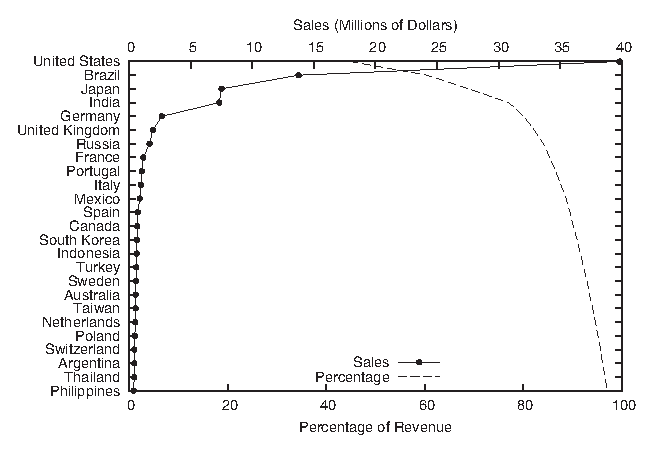
\includegraphics{img/sales}}
  \caption{A rank-order plot of sales per country. The independent
    variable has been plotted along the \emph{vertical} axis to make
    the text labels easier to read.}
  \label{fig:sales}
\end{figure}

Figure \ref{fig:sales} shows the sales by a certain company to
different countries. Not only the sales to each country but also the
cumulative sales are shown, which allows us to assess the importance
of the remaining ``tail'' of the distribution of sales.

In this example, I chose to plot the independent variable along the
vertical axis. This is often a good idea when the values are strings,
since they are easier to read this way. (If you plot them along the
horizontal axis, it is often necessary to rotate the strings by 90
degrees to make them fit, which makes hard to read.)

\begin{figure}
  \centerline{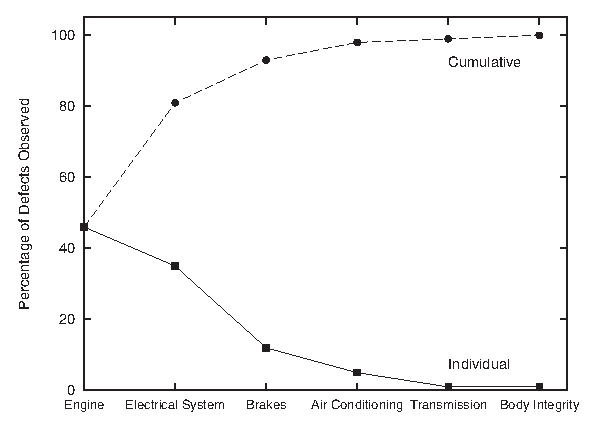
\includegraphics{img/pareto}}
  \caption{The Pareto chart is another example of a rank-order plot.}
  \label{fig:pareto}
\end{figure}

Figure \ref{fig:pareto} displays what in quality engineering is known
as a \emph{Pareto chart}. \index{Pareto charts} In quality engineering and
process improvement,\vadjust{\pagebreak} the goal is to reduce the number of defects in
a certain product or process. You collect all known causes of defects and
observe how often each one occurs. The results can be summarized
conveniently in a chart like the one in Figure \ref{fig:pareto}. Note
that the causes of defects are sorted by their frequency of
occurrence. From this chart we can see immediately that problems with
the engine and the electrical system are much more common than
problems\vadjust{\pagebreak} with the air conditioning, the brakes, or the transmission.
In fact, by looking at the cumulative error curve, we can tell that
fixing just the first two problem areas would reduce the overall
defect rate by 80 percent.

Two more bits of terminology: the term ``Pareto chart'' is not used
widely outside the specific engineering disciplines mentioned in the
previous paragraph. I personally prefer the expression
\emph{rank-order chart} for any plot generated by first sorting all
entries by the dependent variable (\ie, by the \emph{rank} of the
entry). The cumulative distribution curve is occasionally referred to
as a \emph{lift curve}, \index{lift curves} because it tells us how much ``lift'' we get
from each entry or range of entries.
      
\index{univariate analysis!rank-order plots and lift charts|)}
\index{rank-order plots|)}
\index{lift charts|)}

%============================================================
\section{Only When Appropriate: Summary Statistics and Box Plots}

\index{univariate analysis!summary statistics and box plots|(}
   
You may have noticed that so far I have not spoken at all about such
simple topics as mean and median, standard deviation, and 
percentiles.\index{mean!about}\index{median}\index{standard deviation}\index{percentiles} 
That is quite intentional. These \emph{summary statistics} apply only
under certain assumptions and are misleading, if not downright wrong,
if those assumptions are not fulfilled. I know that these quantities
are easy to understand and easy to calculate, but if there is one
message I would like you to take away from this book it is this: the
fact that something is convenient and popular is no reason to follow
suit. For any method that you want to use, make sure you understand
the underlying assumptions and \emph{always} check that they are
fulfilled for the specific application you have in mind!

Mean, median, and related summary statistics apply only to
distributions that have a single, central peak---that is, to
\emph{unimodal} distributions. If this basic assumption is not
fulfilled, then conclusions based on simple summary statistics will be
wrong. Even worse, nothing will tip you off that they are wrong: the
numbers will look quite reasonable. (We will see an example of this
problem shortly.)

\subsection{Summary Statistics}

\index{summary statistics|(}

If a distribution has only a single peak, then it makes sense to ask
about the properties of that peak: where is it located, and what is
its width? We may also want to know whether the distribution is
symmetric and whether any outliers are present.

Mean and standard deviation are two popular measures for location and
spread. The \emph{mean} or average is both familiar and intuitive:
%
\[
m = \frac{1}{n} \sum_i x_i
\]
%
The standard deviation measures how far points spread ``on average''
from the mean: we take all the differences between each individual
point and the mean, and then calculate the average of all these
differences. Because data points can either overshoot or undershoot
the mean and we don't\vadjust{\pagebreak} want the positive and negative deviations to
cancel each other, we sum the \emph{square} of the individual
deviations and then take the mean of the square deviations.  (The
second equation is very useful in practice and can be found from the
first after plugging in the definition of the mean.)
%
\begin{align*}
s^2 & = \frac{1}{n} \sum_i \paren{ x_i - m }^2 \\
    & = \frac{1}{n} \sum_i x_i^2 - m^2
\end{align*}
%
The quantity $s^2$ calculated in this way is known as the
\emph{variance} and is the more important quantity from a theoretical
point of view. But as a measure of the spread of a distribution, we are
better off using its square root, which is known as the \emph{standard
  deviation}. Why take the square root?  Because then both measure for
the location, and the measure for the spread will have the same units,
which are also the units of the actual data. (If our data set consists
of the prices for a basket of goods, then the variance would be given
in ``square dollars,'' whereas the standard deviation would be given
in dollars.)

For many (but certainly not all!) data sets arising in practice, one
can expect about two thirds of all data points to fall within the
interval $[m-s, m+s]$ and 99 percent of all points to fall within the
wider interval $[m-3s, m+3s]$.

Mean and standard deviation are easy to calculate, and have certain
nice mathematical properties---provided the data is symmetric and does
not contain crazy outliers. Unfortunately, many data sets violate at
least one of these assumptions. Here is an example for the kind of
trouble that one may encounter. Assume we have 10 items costing \$1
each, and one item costing \$20. The mean item price comes out to be
\$2.73, even though no item has a price anywhere near this value. The
standard deviation is even~worse: it comes out to \$5.46, implying
that most items have a price between $\text{\$2.73}-\text{\$5.46}$ and
$\text{\$2.73}+\text{\$5.46}$. The ``expected range'' now includes
negative prices---an obviously absurd result. Note that the data set
itself is not particularly pathological: going to the grocery store
and picking up a handful of candy bars and a bottle of wine will do it
(pretty good wine, to be sure, but nothing outrageous).

A different set of summary statistics that is both more flexible and
more robust is based on the concepts of \emph{median}\index{median} and
\emph{quantiles}\index{quantiles} or \emph{percentiles}.\index{percentiles} The median is conventionally
defined as the value from a data set such that half of all points in
the data set are smaller and the other half greater that that value.
Percentiles are the generalization of this concept to other fractions
(the 10th percentile is the value such that 10 percent of all points
in the data set are smaller than it, and so on).  Quantiles are
similar to percentiles, only that they are taken with respect to the
fraction of points, not the percentage of points (in other words, the
10th percentile equals the 0.1 quantile).

Simple as it is, the percentile concept is nevertheless ambiguous, and
so we need to work a little harder to make it really concrete. As an
example of the problems that occur, consider the data set $\braces{ 1,
  2, 3 }$. What is the median?\vadjust{\pagebreak} It is not possible to break this data
set into two equal parts each containing exactly half the points. The
problem becomes even more uncomfortable when we are dealing with
arbitrary percentile values (rather than the median only).

The Internet standard laid down in RFC 2330 (``Framework for IP
Performance Metrics'') gives a definition of percentiles in terms of
the CDF, which is unambiguous and practical, as follows.  The $p$th
percentile is the smallest value $x$, such that the cumulative
distribution function of $x$ is greater or equal $p/100$.
\[
\text{$p$th percentile: smallest $x$ for which }
\operatorname{cdf}(x) \ge p/100
\]
This definition assumes that the CDF is normalized to 1,
not to 100. If it were normalized to 100, the condition would be
$\operatorname{cdf}(x) \ge p$.

With this definition, the median (\ie, the 50th percentile) of the
data set $\braces{1,2,3}$ is $2$ because the $\operatorname{cdf}(1) =
0.33\dots$, $\operatorname{cdf}(2) = 0.66\dots$, and
$\operatorname{cdf}(3) = 1.0$.  The median of the data set
$\braces{1,2}$ would be $1$ because now $\operatorname{cdf}(1) = 0.5$,
and $\operatorname{cdf}(2) = 1.0$.

The median is a measure for the location of the distribution, and we
can use percentiles to construct a measure for the width of the
distribution. Probably the most frequently used quantity for this
purpose is the \emph{inter-quartile range} (IQR), which is the
distance between the 75th percentile and 25th percentile.

When should you favor median and percentile over mean and standard
deviation? Whenever you suspect that your distribution is not
symmetric or has important outliers.

If a distribution is symmetric and well behaved, then mean and median
will be quite close together, and there is little difference in using
either. Once the distribution becomes skewed, however, the basic
assumption that underlies the mean as a measure for the location of
the distribution is no longer fulfilled, and so you are better off
using the median. (This is why the average wage is usually given in
official publications as the median family income, not the mean; the
latter would be significantly distorted by the few households with
extremely high incomes.) Furthermore, the moment you have outliers,
the assumptions behind the standard deviation as a measure of the
width of the distribution are violated; in this case you should favor
the IQR (recall our shopping basket example earlier).

If median and percentiles are so great, then why don't we always use
them?  A large part of the preference for mean and variance is
historical. In the days before readily available computing power,
percentiles were simply not practical to calculate. Keep in mind that
finding percentiles requires to \emph{sort} the data set whereas to
find the mean requires only to add up all elements in any order. The
latter is an $\mathcal{O}(n)$ process, but the former is an
$\mathcal{O}(n^2)$ process, since humans---being nonrecursive---cannot
be taught Quicksort and therefore need to resort to much less
efficient sorting algorithms. A second reason is that it is much harder
to prove rigorous theorems for percentiles, whereas mean and variance
are mathematically very well behaved and easy to work with.

\index{summary statistics|)}

\subsection{Box-and-Whisker Plots}

\index{box-and-whisker plots!about|(}

There is an interesting graphical way to represent these quantities,
together with information about potential outliers, known as a
\emph{box-and-whisker plot}, or \emph{box plot} for short. Figure
\ref{fig:glassboxplot} illustrates all components of a box plot. A box
plot consists of:

\begin{itemize}
\item A \emph{marker} or symbol for the median as an indicator of the
  \emph{location} of the distribution

\item A \emph{box}, spanning the inter-quartile range, as a measure of
  the \emph{width} of the distribution

\item A set of \emph{whiskers}, extending from the central box to the
  upper and lower adjacent values, as an indicator of the \emph{tails}
  of the distribution (where ``adjacent value'' is defined in the next
  paragraph)

\item Individual \emph{symbols} for all values outside the range of
  adjacent values, as a representation for \emph{outliers}
\end{itemize}

You can see that a box plot combines a lot of information in a single
graph. We have encountered almost all of these concepts before, with
the exception of upper and lower \emph{adjacent values}. While the
inter-quartile range is a measure for the width of the central
``bulk'' of the distribution, the adjacent values are one possible way
to express how far its tails reach.  The upper adjacent value is the
largest value in the data set that is less than twice the
inter-quartile range greater than the median. In other words: extend
the whisker upward from the median to twice the length of the central
box. Now trim the whisker down to the largest value that actually
occurs in the data set; this value is the upper adjacent value. (A
similar construction holds for the lower adjacent value.)

You may wonder about the reason for this peculiar construction. Why
not simply extend the whiskers to, say, the 5th and 95th percentile
and be done with it? The problem with this approach is that it does
not allow us to recognize true outliers! Outliers are data points that
are, \emph{when compared to the width of the distribution}, unusually
far from the center. Such values may or may not be present.  The top
and bottom 5 percent, on the other hand, are always present even for
very compact distributions. To recognize outliers, we therefore cannot
simply look at the most extreme values, instead we must \emph{compare
  their distance from the center to the overall width of the
  distribution}.  That is what box-and-whisker plots, as described in
the previous paragraph, do.

The logic behind the preceding argument is extremely important (not
only in this application but more generally), so I shall reiterate the
steps: \emph{first} we calculated a measure for the width of the
distribution, \emph{then} we used this width to identify outliers as
those points that are far from the center, where (and this is the
crucial step) ``far'' is measured in units of the width of the
distribution. We neither impose an arbitrary distance from the
outside, nor do we simply label the most extreme $x$ percent of the
distribution as outliers---instead, we determine the width of the
distribution (as the range into which points ``typically'' fall) and
then use it to identify outliers as those points that deviate from
this range.  The important insight here is that the distribution
itself determines a typical \emph{scale}, which provides a natural
unit in which\vadjust{\pagebreak} to measure other properties of the distribution. This
idea of using some typical property of the system to describe other
parts of the system will come up again later (see Chapter
\ref{ch:scaling}).

Box plots combine many different measures of a distribution into a
single, compact graph. A box plot allows us to see whether the
distribution is symmetric or not and how the weight is distributed
between the central peak and the tails. Finally, outliers (if present)
are not dropped but shown explicitly.

Box plots are best when used to compare several distributions against
one another---for a single distribution, the overhead of preparing
and managing a graph (compared to just quoting the numbers) may often 
not appear justified. Here is an example that compares different data
sets against each other.

Let's say we have a data set containing the index of refraction of 121
samples of glass.\footnote{The raw data can be found in the ``Glass
  Identification Data Set'' on the UCI Machine Learning Repository at
  \url{http://archive.ics.uci.edu/ml/}.} The data
set is broken down by the type of glass: 70 samples of window glass,
29 from headlamps, 13 from containers of various kinds, and 9 from
tableware. Figures \ref{fig:glasskde} and \ref{fig:glassboxplot} are
two representations of the same data, the former as a kernel density
estimate and the latter as a box plot.

The box plot emphasizes the overall structure of the data sets and
makes it easy to compare the data sets based on their location and
width. At the same time, it also loses much information. The KDE gives
a more detailed view of the data---in particular showing the
occurrence of multiple peaks in the distribution functions---but makes
it more difficult to quickly sort and classify the data sets.
Depending on your needs, one or the other technique may be preferable
at any given time.

Here are some additional notes on box plots.

\begin{itemize}
\item The specific way of drawing a box plot that I described here is
  especially useful but is far from universal. In particular, the
  specific definition of the adjacent values is often not properly
  understood. Whenever you find yourself looking at a box plot, always
  ask what exactly is shown, and whenever you prepare one, make sure
  to include an explanation.

\item The box plot described here can be modified and enhanced.  For
  example, the width of~the central box (\ie, the direction orthogonal
  to the whiskers) can be used to indicate the size of the underlying
  data set: the more points are included, the wider the box. Another
  possibility is to abandon the rectangular shape of the box
  altogether and to use the local width of the box to display the
  density of points at each location---\break which brings us almost full
  circle to KDEs.
\end{itemize}

\index{univariate analysis!summary statistics and box plots|)}
\index{box-and-whisker plots!about|)}


\begin{figure}
  \centerline{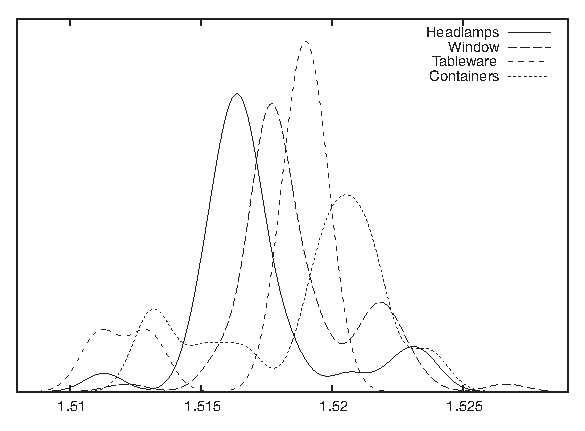
\includegraphics{img/glass-kde}}
  \caption{Comparing data sets using KDEs: refractive index of different
    types of glass. (Compare Figure \ref{fig:glassboxplot}.)}
  \label{fig:glasskde}\vspace*{-6pt}
\end{figure} 

% ============================================================
\section{Workshop: NumPy}

\index{NumPy|(}
\index{software!NumPy|(}
 
The NumPy module provides efficient and convenient handling of large
numerical arrays in Python.  It is the successor to both the earlier
Numeric and the alternative numarray modules. (See the Appendix
\ref{app:tools} for more on the history of scientific computing with
Python.) The NumPy module is used by many other libraries and projects
and in this sense is a ``base'' technology.

\begin{figure}
\vspace*{-6pt}
  \centerline{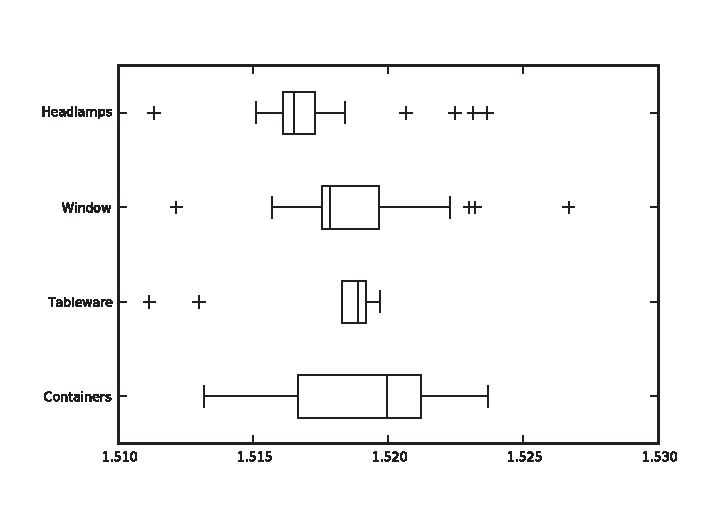
\includegraphics{img/glass-boxplot}}\vspace*{-6pt}
  \caption{Comparing data sets using box plots: refractive index of 
    different types of glass. (Compare Figure \ref{fig:glasskde}.)}
  \label{fig:glassboxplot}\vspace*{-6pt}
\end{figure}

Let's look at some quick examples before delving a bit deeper into
technical details.

\vspace*{-9pt}
\subsection{NumPy in Action}

NumPy objects are of type \texttt{ndarray}.  There are different ways
of creating them. We can create an \texttt{ndarray} by:

\begin{itemize}
\item Converting a Python list
\item Using a factory function that returns a populated vector
\item Reading data from a file directly into a NumPy object
\end{itemize}

The listing that follows shows five different ways to create NumPy
objects.  First we create one by converting a Python list. Then we
show two different factory routines that generate equally spaced grid
points.  These routines differ in how they interpret the provided
boundary values: one routine includes both boundary values, and the
other includes one and excludes the other. Next we create a vector
filled with zeros and set each element\vadjust{\pagebreak} in a loop. Finally, we read
data from a text file.  (I am showing only the simplest or default
cases here---all these routines have many more options that can be
used to influence their behavior.)

\begin{verbatim}
# Five different ways to create a vector...

import numpy as np

# From a Python list
vec1 = np.array( [ 0., 1., 2., 3., 4. ] )
\end{verbatim}

\begin{verbatim}
# arange( start inclusive, stop exclusive, step size )
vec2 = np.arange( 0, 5, 1, dtype=float )

# linspace( start inclusive, stop inclusive, number of elements )
vec3 = np.linspace( 0, 4, 5 )

# zeros( n ) returns a vector filled with n zeros
vec4 = np.zeros( 5 )
for i in range( 5 ):
    vec4[i] = i

# read from a text file, one number per row
vec5 = np.loadtxt( "data" )
\end{verbatim}

In the end, all five vectors contain identical data.  You should
observe that the values in the Python list used to initialize
\texttt{vec1} are floating-point values and that we specified the
\emph{type} desired for the vector elements explicitly when using the
\texttt{arange()} function to create \texttt{vec2}. (We will come back
to types in a moment.)

Now that we have created these objects, we can operate with them (see
the next listing). One of the major conveniences provided by NumPy is
that we can operate with NumPy objects as if they were atomic data
types: we can add, subtract, and multiply them (and so forth)
\emph{without the need for explicit loops}. Avoiding explicit loops
makes our code clearer. It also makes it faster (because the entire
operation is performed in C without overhead--- see the discussion that
follows).

\begin{verbatim}
# ... continuation from previous listing

# Add a vector to another
v1 = vec1 + vec2

# Unnecessary: adding two vectors using an explicit loop
v2 = np.zeros( 5 )
for i in range( 5 ):
    v2[i] = vec1[i] + vec2[i]

# Adding a vector to another in place
vec1 += vec2

# Broadcasting: combining scalars and vectors
v3 = 2*vec3
v4 = vec4 + 3

# Ufuncs: applying a function to a vector, element by element
v5 = np.sin(vec5)

# Converting to Python list object again
lst = v5.tolist()
\end{verbatim}

All operations are performed element by element: if we add two
vectors, then the corresponding elements from each vector are combined
to give the element in the resulting vector. In other words, the
compact expression \texttt{vec1 + vec2} for \texttt{v1} in the listing
is equivalent to the explicit loop construction used to calculate
\texttt{v2}. This is true even for multiplication: \texttt{vec1 *
  vec2} will result in a vector in which the corresponding elements of
both operands have been multiplied element by element. (If you want a
true vector or ``dot'' product, you must use the \texttt{dot()}
function instead.) Obviously, this requires that \emph{all operands
  have the same number of elements}!

Now we shall demonstrate two further convenience features that in the
NumPy documentation are referred to as \emph{broadcasting} \index{broadcasting, NumPy} and
\emph{ufuncs} (short for ``universal functions''). \index{ufuncs (universal functions), NumPy} The term
``broadcasting'' in this context has nothing to do with messaging.
Instead, it means that if you try to combine two arguments of
different shapes, then the smaller one will be extended (``cast
broader'') to match the larger one. This is especially useful when
combining scalars with vectors: the scalar is expanded to a vector of
appropriate size and whose elements all have the value given by the
scalar; then the operation proceeds, element by element, as before.
The term ``ufunc'' refers to a scalar function that can be applied to
a NumPy object. The function is applied,\vadjust{\pagebreak} element by element, to all
entries in the NumPy object, and the result is a new NumPy object with
the same shape as the original one.

Using these features skillfully, a function to calculate a kernel
density estimate can be written as a \emph{single} line of code:

\begin{verbatim}
# Calculating kernel density estimates

from numpy import *

# z: position, w: bandwidth, xv: vector of points
def kde( z, w, xv ):
    return sum( exp(-0.5*((z-xv)/w)**2)/sqrt(2*pi*w**2) )

d = loadtxt( "presidents", usecols=(2,) )

w = 2.5

for x in linspace( min(d)-w, max(d)+w, 1000 ):
    print x, kde( x, w, d )
\end{verbatim}

This program will calculate and print the data needed to generate
Figure \ref{fig:presidentskde} (but it does not actually draw the
graph---that will have to wait until we introduce \texttt{matplotlib}
in the Workshop of Chapter \ref{ch:bivariate}).

Most of the listing is boilerplate code, such as reading and writing
files.  All the actual work is done in the one-line function
\texttt{kde(z, w, xv)}. This function makes use of both
``broadcasting'' and ``ufuncs'' and is a good example for the style of
programming typical of NumPy. Let's dissect it---inside out.

First recall what we need to do when evaluating a KDE: for each
location $z$ at which we want to evaluate the KDE, we must find its
distance to all the points in the data set. For each point, we
evaluate the kernel for this distance and sum up the contributions
from all the individual kernels to obtain the value of the KDE at $z$.

The expression \texttt{z-xv} generates a vector that contains the
distance between \texttt{z} and all the points in \texttt{xv} (that's
broadcasting). We then divide by the required bandwidth, multiply by
$1/2$, and square each element. Finally, we apply the exponential
function \texttt{exp()} to this vector (that's a ufunc).  The result
is a vector that contains the exponential function evaluated at the
distances between the points in the data set and the location
\texttt{z}.  Now we only need to sum all the elements in the vector
(that's what \texttt{sum()} does) and we are done, having calculated
the KDE at position \texttt{z}. If we want to plot the KDE as a curve,
we have to repeat this process for each location we wish to
plot---that's what the final loop in the listing is for.

\vspace*{-6pt}
\subsection{NumPy in Detail}

You may have noticed that none of the warm-up examples in the listings
in the previous section contained any matrices or other data
structures\vadjust{\pagebreak} of higher dimensionality---just one-dimensional vectors.
To understand how NumPy treats objects with dimensions greater than one,
we need to develop at least a superficial understanding for the way
NumPy is implemented.

It is misleading to think of NumPy as a ``matrix package for Python''
(although it's commonly used as such). I find it more helpful to think
of NumPy as a wrapper and access layer for underlying C buffers.
These buffers are contiguous blocks of C memory, which---by their
nature---are one-dimensional data structures. All elements in those
data structures must be of the same size, and we can specify almost
any native C type (including C structs) as the type of the individual
elements. The default type corresponds to a C \texttt{double} and that
is what we use in the examples that follow, but keep in mind that
other choices are possible. All operations that apply to the data
overall are performed in C and are therefore very fast.

To interpret the data as a matrix or other multi-dimensional data
structure, the shape or layout is imposed during element access.  The
same $12$-element data structure can therefore be interpreted as a
$12$-element vector or a $3\times 4$ matrix or a $2 \times 2 \times 3$
tensor---the shape comes into play only through the way we access the
individual elements. (Keep in mind that although reshaping a data
structure is very easy, resizing is not.)

The encapsulation of the underlying C data structures is not perfect:
when choosing the types of the atomic elements, we specify C data
types not Python types. Similarly, some features provided by NumPy
allow us to manage memory manually, rather than have the memory be
managed transparently by the Python runtime. This is an intentional
design decision, because NumPy has been designed to accommodate
\emph{large} data structures---large enough that you might want (or
need) to exercise a greater degree of control over the way memory is
managed. For this reason, you have the ability to choose types that
take up less space as elements in a collection (\eg, C \texttt{float}
elements rather than the default \texttt{double}). For the same
reason, all ufuncs accept an optional argument pointing to an (already
allocated) location where the results will be placed, thereby avoiding
the need to claim additional memory themselves. Finally, several
access and structuring routines return a \emph{view} (not a copy!) of
the same underlying data. This does pose an aliasing problem that you
need to watch out for.

The next listing quickly demonstrates the concepts of shape and views.
Here, I assume that the commands are entered at an interactive Python
prompt (shown as \texttt{>>>} in the listing).  Output generated by
Python is shown without a prompt:

\begin{verbatim}
>>> import numpy as np

>>> # Generate two vectors with 12 elements each
>>> d1 = np.linspace( 0, 11, 12 )
>>> d2 = np.linspace( 0, 11, 12 )

>>> # Reshape the first vector to a 3x4 (row x col) matrix
>>> d1.shape = ( 3, 4 )
>>> print d1
\end{verbatim}
\begin{verbatim}
[[  0.   1.   2.   3.]
 [  4.   5.   6.   7.]
 [  8.   9.  10.  11.]]

>>> # Generate a matrix VIEW to the second vector
>>> view = d2.reshape( (3,4) )

>>> # Now: possible to combine the matrix and the view
>>> total = d1 + view


>>> # Element access: [row,col] for matrix
>>> print d1[0,1]
1.0
>>> print view[0,1]
1.0
>>> # ... and [pos] for vector
>>> print d2[1]
1.0


>>> # Shape or layout information
>>> print d1.shape
(3,4)
>>> print d2.shape
(12,)
>>> print view.shape
(3,4)

>>> # Number of elements (both commands equivalent)
>>> print d1.size
12
>>> print len(d2)
12

>>> # Number of dimensions (both commands equivalent)
>>> print d1.ndim
2
>>> print np.rank(d2)
1
\end{verbatim}

Let's step through this. We create two vectors of 12 elements each.
Then we \emph{reshape} the first one into a $3 \times 4$ matrix. Note
that the \texttt{shape} property is a data member---not an accessor
function! For the second vector, we create a \emph{view} in the form
of a $3 \times 4$ matrix. Now \texttt{d1} and the newly created view
of \texttt{d2} have the same shape, so we can combine them (by forming
their sum, in this case). Note that even though \texttt{reshape()} is
a member function, it does \emph{not} change the shape of the instance
itself but instead returns a new view object: \texttt{d2} is still a
one-dimensional vector. (There is also a standalone version of this
function, so we could also have written \texttt{view = np.reshape( d2,
  (3,4) )}. The presence of such redundant functionality is due to the
desire to maintain backward compatibility with both of NumPy's
ancestors.)

We can now access individual elements of the data structures,
depending on their shape. Since both \texttt{d1} and \texttt{view} are
matrices, they are indexed by a pair of indices (in the order
\texttt{[row,col]}). However, \texttt{d2} is still a one-dimensional
vector and thus takes only a single index. (We will have more to say
about indexing in a moment.)

Finally, we examine some diagnostics regarding the shape of the data
structures, emphasizing their precise semantics.  The \texttt{shape}
is a tuple, giving the number of elements in each dimension. The
\texttt{size} is the total number of elements and corresponds to the
value returned by \texttt{len()} for the entire data structure.
Finally, \texttt{ndim} gives the number of dimensions (\ie,
\texttt{d.ndim == len(d.shape)}) and is equivalent to the ``rank'' of
the entire data structure. (Again, the redundant functionality exists
to maintain backward compatibility.)

Finally, let's take a closer look at the ways in which we can access
elements or larger subsets of an \texttt{ndarray}. In the previous
listing we saw how to access an individual element by fully specifying
an index for each dimension.  We can also specify larger subarrays of
a data structure using two additional techniques, known as
\emph{slicing} \index{slicing, NumPy} and \emph{advanced indexing}. \index{advanced indexing, NumPy} The following listing
shows some representative examples. (Again, consider this an
interactive Python session.)

\begin{verbatim}
>>> import numpy as np

>>> # Create a 12-element vector and reshape into 3x4 matrix
>>> d = np.linspace( 0, 11, 12 )
>>> d.shape = ( 3,4 )
>>> print d
[[  0.   1.   2.   3.]
 [  4.   5.   6.   7.]
 [  8.   9.  10.  11.]]

>>> # Slicing...
>>> # First row
>>> print d[0,:]
[ 0.  1.  2.  3.]

>>> # Second col
>>> print d[:,1]
[ 1.  5.  9.]

>>> # Individual element: scalar
>>> print d[0,1]
1.0

>>> # Subvector of shape 1
>>> print d[0:1,1]
[ 1.]

>>> # Subarray of shape 1x1
>>> print d[0:1,1:2]
[[ 1.]]
\end{verbatim}

\begin{verbatim}
>>> # Indexing...
>>> # Integer indexing: third and first column
>>> print d[ :, [2,0] ]
[[  2.   0.]
 [  6.   4.]
 [ 10.   8.]]

>>> # Boolean indexing: second and third column
>>> k = np.array( [False, True, True] )
>>> print d[ k, : ]
[[  4.   5.   6.   7.]
 [  8.   9.  10.  11.]]
\end{verbatim}\vspace*{-3pt}

We first create a $12$-element vector and reshape it into a $3 \times
4$ matrix as before. Slicing uses the standard Python slicing syntax
\texttt{start:stop:step}, where the start position is inclusive but
the stopping position is exclusive. (In the listing, I use only the
simplest form of slicing, selecting all available elements.)

There are two potential ``gotchas'' with slicing. First of all,
specifying an explicit subscripting index (not a slice!) reduces the
corresponding dimension to a scalar.  Slicing, though, does not reduce
the dimensionality of the data structure. Consider the two extreme
cases: in the expression \texttt{d[0,1]}, indices for both dimensions
are fully specified, and so we are left with a scalar. In contrast,
\texttt{d[0:1,1:2]} is sliced in both dimensions. Neither dimension is
removed, and the resulting object is still a (two-dimensional) matrix
but of smaller size: it has shape $1 \times 1$.

The second issue to watch out for is that \emph{slices return views},
not copies.

Besides slicing, we can also index an \texttt{ndarray} with a vector
of indices, by an operation called ``advanced indexing.'' The previous
listing showed two simple examples. In the first we use a Python list
object, which contains the integer indices (\ie, the positions) of the
desired columns and in the desired order, to select a subset of
columns. In the second example, we form an \texttt{ndarray} of Boolean
entries to select only those rows for which the Boolean evaluates to
True.

In contrast to slicing, \emph{advanced indexing returns copies}, not
views.

% Finally, be careful when using tuples for indexing: WHY?
% http://docs.scipy.org/doc/numpy/reference/arrays.indexing.html

This completes our overview of the basic capabilities of the NumPy
module. NumPy is easy and convenient to use for simple use cases but
can get very confusing otherwise. (For example, check out the rules for
general broadcasting when both operators are multi-dimensional, or for
advanced indexing).

We will present some more straightforward applications in Chapters
\ref{ch:bivariate} and \ref{ch:timeseries}.
      
% ============================================================
% \section{Summary}
% 
% This concludes our survey of methods to study univariate data. The
% most important questions when exploring univariate data sets concern
% the overall shape of the distribution of points; and, more
% specifically, its location and shape.
% 
% We looked at simple graphical methods, such as dot and jitter plots,
% and at more sophisticated methods, such as histograms and kernel
% density estimates, which allows us to discern more detail about the
% data. I stressed the importance of cumulative distribution functions,
% which --- although less intuitive than a simple histogram ---
% nevertheless allow us to make quantitative statements about the
% distribution of points.
% 
% Finally, I introduced summary statistics, such as mean, median, and so
% on, and discussed their limitations. We also learned about box plots
% as a compact method to compare several data sets against each other.
% 
% We also introduced some more advanced or specialized techniques, such
% as rank-order plots (for data sets where the independent variable has
% not specific ordering), and QQ-plots, which can be used to determine
% if two data sets have the same distribution.
  
\index{NumPy|)}
\index{software!NumPy|)}


\vspace*{-9pt}
% ============================================================
\section{Further Reading}

\begin{itemize}
\item \cit{The Elements of Graphing Data}{William S.\ Cleveland}{2nd ed.,
    Hobart Press}{1994}
  A book-length discussion of graphical methods for data analysis such
  as those described in this chapter. In particular,\vadjust{\pagebreak} you will find
  more information here on topics such as box~plots and QQ plots.
  Cleveland's methods are particularly careful and well thought-out.

\item \cit{All of Statistics: A Concise Course in Statistical 
    Inference}{Larry Wasserman}{Springer}{2004}
  A thoroughly modern treatment of mathematical statistics, very 
  advanced and condensed. You will find some additional material 
  here on the theory of ``density estimation''---that is, on histograms
  and KDEs.

\item \cit{Multivariate Density Estimation}{David W.\ Scott}{2nd ed.,
    Wiley}{2006}
  A research monograph on density estimation written by the creator of
  Scott's rule.

\item \cit{Kernel Smoothing}{M.\ P.\ Wand and M.\ C.\ Jones}{Chapman \& 
    Hall}{1995}
  An accessible treatment of kernel density estimation.
\end{itemize}

\index{data analysis!univariate analysis|)}
\index{univariate analysis|)}
